% !TEX root = ../thesis.tex
{\usekomafont{chapter}Résumé substentiel}


\section*{Contexte} % (fold)

De la même manière que le LHC est une plate-forme expérimentale pour explorer la mécanique quantique et mieux comprendre ce qu’est notre univers, les humanoïdes peuvent servir de simulateurs simplifiés et surtout parametrables de l'Homme. Ainsi, les robots humanoïdes peuvent devenir des outils incroyables pour étudier les êtres humains et, éventuellement, contribuer à une meilleure compréhension du comportement et des capacités de l’homme~(\cite{atkeson2000using}, \cite{cheng2007cb}, \cite{brooks1986achieving}, \cite{oudeyer2010impact}).

Un exemple célèbre de ce type  d’utilisation a été le projet Cog~\parencite{brooks1999cog} à l'Humanoid Robotics Group de l'Institut de Technologie du Massachusetts(MIT). Ce projet de recherche avait deux objectifs: un objectif d'ingénierie de construction d'un prototype polyavelent de robot autonome, compliant et adroit, ainsi qu’un objectif scientifique de la compréhension de la cognition humaine~\parencite{brooks1994building}. Dans ce but, ils ont construit plusieurs plate-formes robotiques dont un humanoïde~\parencite{brooks1999cog}, et une tête multi-articulé très expressive nommé Kismet~\parencite{breazeal2003emotion}.

Cette thèse est fondée sur les mêmes motivations scientifiques que le travail de R. Brooks, R. Pfeifer, T. McGeer et les initiatives comme le projet Cog c’est-à-dire \textbf{explorer le rôle de la morphologie, de la cognition et de l'intelligence incarnée à travers l'utilisation de plates-formes robotiques expérimentales interagissant avec le monde réel}.

L'approche scientifique des robots Cog est orientée vers l'exploration du rôle du corps sur plusieurs niveaux: la mécatronique, le système de controle, le design de la tête...  mais ces robots ont été construits il y a plus de 15 ans, les techniques de productions utilisées, les rendent coûteux, compliqués à modifier et particulièrement difficiles à diffuser dans d'autres laboratoires.

Nous sommes maintenant en 2014, la révolution des makers est en cours~\parencite{anderson2012makers} et de nouvelles technologies permettent de repenser la façon dont nous concevons les plates-formes robotiques, en particulier celles humanoïdes.


Dans notre équipe, Inria Flowers\footnote{\url{flowers.inria.fr}}, nous sommes intéressés par l'étude des mécanismes qui peuvent permettre à des robots et aux humains d'acquérir de façon autonome et cumulativement des répertoires de nouvelles compétences sur des périodes de temps prolongées. Cela comprend des mécanismes d'apprentissages par l'auto-exploration, ainsi que l'apprentissage par interaction avec ses pairs, l'acquisition simultanée de compétences sensori-motrices (par exemple la locomotion, l'apprentissage d'affordances et la manipulation active) et de compétences sociales (par exemple, la compréhension du langage, des protocoles d'interaction adaptatifs , et la collaboration homme-robot).

Parmi les questions qui nous interessent particulièrement, une évolution intéressante au cours des dernières décennies a été la démonstration de l'importance de la morphologie des robots pour le contrôle sensori-moteur, la cognition et développement~(\cite{kaplan2008corps} \cite{steels1995artificial} \cite{Pfeifer06}). En effet, le comportement réel d'un robot résulte d'une interaction complexe entre l'algorithme de contrôle, la morphologie du robot et l'environnement~\parencite{Steels1991emergence} dans lequel il agit. En outre, il est clair qu’une morphologie  robotic adaptée, utilisant des propriétés spécifiques permet de réduire considérablement la complexité d'une tâche donnée en assurant implicitement une partie -ou l’integralité- du contrôle nécessaire~\parencite{pfeifer2005morphological}.
Enfin, comme Rodney Brooks le souligne, \emph{le monde est le meilleur modèle de lui même}~\parencite{brooks1991intelligence} et les simulateurs ne peuvent pas \emph{(pour le moment)} gérer de façon réaliste la complexité de la physique réelle avec contacts multiples, des matériaux souples, les frottements ou les interactions multimodales imprévues.


\section*{Objectifs de cette thèse} % (fold)

Malheureusement les plates-formes robotiques actuelles ne sont pas adaptées pour relever ces défis. D'un côté, les robots commerciaux tels que Nao \parencite{gouaillier2008nao}, Darwin Op \parencite{ha2011development}, Nimbro Op \parencite{schwarznimbro} ou iCub \parencite{metta2008icub} sont facilement accessibles et faciles à utiliser. Cependant, ils disposent d’une morphologie «traditionnelle» (ex: une compliance limitée, un torse rigide, de grands pieds, moteurs lourds et puissants) mais surtout, la modification de leurs morphologies est difficile ou impossible.
D’un autre côté, les prototypes de laboratoire~(\cite{wisse2007passive}, \cite{nakanishi2013design}, \cite{ly2011bio}, \cite{niiyama2010athlete}, \cite{radkhah2011concept}) sont principalement produits et optimisés manuellement ce qui les rend presque impossible à reproduire dans un autre laboratoire. En outre, dans la plupart des cas, ils ne sont pas open source et/ou est trop compliqué/coûteux à modifier.

Le principal problème de ces robots est l’approche et les technologies choisies pour les concevoir et les produire. En effet, la façon classique de concevoir et de produire des robots est un processus extrêmement compliqué et coûteux qui implique la fabrication d’outillages spécifiques et l'utilisation de procédés de productions industriels.

Dans cette thèse, nous \textbf {proposons de nouvelles approches et processus de conception pour créer et produire des plates-formes robotiques dont le contrôle et la morphologie peuvent être explorés librement et expérimentés dans le monde réel, tout en étant faciles à diffuser et reproduire dans le milieu académique}. En particulier, cette méthodologie de conception alternative est motivée par le désir de:
\begin{itemize}
    \item explorer librement n'importe quelle propriété morphologique,
    \item réduire la quantité de temps nécessaire entre l'idée et son expérimentation sur une plate-forme robotique réelle et dans le monde réel,
    \item faire que des expériences qui devraient être facile à faire, soit effectivement facile à faire,
    \item rendre le travail et les résultats facilement reproductibles dans tout autre laboratoire,
    \item créer des outils modulaires et libres d'utilisations selon les principes open source, afin qu’il puisse être réutilisés et étendus par d'autres projets.
\end{itemize}


\section*{L'approche Poppy}

Pour atteindre ces objectifs, nous avons décidé de suivre de nouvelles méthodes de conception et de production, et ce, pour tous les aspects technologiques du robot (mécanique, actionneur, électronique, logiciels, distribution). En particulier, ces méthodes s'appuient sur:


\begin{description}
  \item[Structure mécanique:] Nous utilisons exclusivement l'impression 3D (technique de production numérique par ajout de matière) qui offre de multiples avantages pour nos applications, et en particulier son faible coût pour la production unitaire, sa rapidité, son accessibilité à tous (imprimante low cost ou sous traitance) et surtout il s'agit une technique facilement reproductible car numérique, il n'y a pas besoin de posséder de compétence particulière pour faire la production des pièces. 

  Au délà des aspects pratiques, l'impression 3D permet de produire avec differents materiaux et ouvre aussi de nouvelles possibilités en terme de design car il est possible de produire des formes qui étaient impossibles avec les techniques de production classiques. De plus, le coût de production ne dépend plus de la complexité de la pièce mais juste de son gabarit et volume. 
  Il est alors possible d'optimiser au maximum les formes sans se soucier ni des coûts, ni de la faisabilité.

  \item[Senseurs:] Avec l'électronique, nous n'avons pas la même liberté de production rapide, low cost et unitaire. Nous avons choisis d'utiliser l'environement Arduino. Ainsi toute l'acquisition des senseurs des robots Poppy est fait en utilisant des cartes Arduino (ou compatible). Elles offrent beaucoup d'entrées/sorties (numériques, analogique, bus de communication série) associées à un environnement de programmation très simple qui permet, sans aucune connaissance bas niveau sur les architectures de micro-controller de facilement interargir avec des composants electroniques.
  De plus c'est un projet open source qui a 10 ans, il y aune grosse communauté et beaucoup de developpements ont été fait, donnant accès à un grand catalogue de capteur low-cost prêt à utiliser.

  Ainsi, il devient possible d'explorer assez librement differents types et positionnement de senseurs pour modifier l'appareil sensitif d'un robot.

  \item[Actionneurs:] Pour la motorisation, nous avons decidé d'utiliser les actuateurs Robotis Dynamixels car ils se présentent sous la forme d'un module tout-en-un (disponible en differentes puissances) qui inclu une mécanique de qualité (moteur Maxon et engrennages en métal) ainsi qu'une carte electronique assurant le contrôle bas niveau et la mise en réseau via un bus, permetttant de brancher tous les actuateurs en série. Ces modules permettent de réduire la complexité de l'assemblage et le nombre de fils tout en restant relativement accessibles (environ 200€/unit).

  De plus, il est possible d'ajuster dynamiquement la compliance, ce qui permet l'exploration de mouvements souples ou passifs.

  \item[Contrôle:] Nous avons conçu une nouvelle bibliothèque de contrôle sensori-moteur robuste et modularisée appelée pypot. Nous nous sommes focalisés sur la conception d'une API intuitive et modulaire, permetttant un accès et un contrôle simplifiés à tous les composants d'un robot aux moteurs et aux senseurs, et qui inclus des primitives combinables pour la construction de synergies.

  Nous avons choisis d'utiliser Python, car ce langage permet un développement rapide, un déploiement facile sur tous les systèmes d'exploitation et un simplicité dans l'écriture des scripts pour des développeurs non experts. Il offre également une grande variété de bibliothèques scientifiques et machine-learning utilisées en robotique (par exemple Numpy, Scipy, scikit-learn).

  Cette bilbiothèque est entièrement documentés (voir: \url{http://poppy-project.github.io/pypot/}).
  
  \item[Open source:] Enfin, comme l'aspect principal d'une telle approche est de permettre la variabilité, la réutilisation et la modification de la conception initiale, \textbf{il est nécessaire} de diffuser non seulement notre travail à travers des publications scientifiques mais aussi de distribuer le matériel nécessaire. 
  Cela signifie que quiconque à l'extérieur de notre laboratoire devrait avoir accès aux sources et être libre de faire les changements appropriés à sa propre recherche. Par conséquent, en plus des choix technologiques présentés précédemment, nous avons la politique de distribuer la totalité de notre travail (logiciels et matériel) sous des licences open source. Ceci est un aspect fondamental vers la construction de nouveaux outils de recherche qui facilitent à la fois la reproductibilité des résultats scientifiques et plus généralement favorise la pratique de science cumulative en robotique.

  \item[Communautaire:] Un dernier point important et pourtant rarement mis en avant dans les travaux scientifiques est la création d'une communauté et d'outils d'échanges. Il s'agit de faciliter le travail collaboratif et multi-disciplinaire, de faciliter le support et le debug tout en favorisant les échanges d'idées. 

  Pour cela nous utilisons 2 outils principaux: GitHub\footnote{\url{https://www.github.com/poppy_project/}} pour de developpement technologique et Discourse\footnote{\url{https://forum.poppy-project.org}} pour heberger toutes les discussions et projets.

\end{description}

En utilisant cette approche, une premier robot humanoide complet a été developpé et utilisé dans plusieurs applications. Poppy est le premier robot humanoide complet à être à la fois imprimé en 3D et open source. 


\section*{L'humanoide Poppy} % (fold)

Poppy Humanoïde (voir~Fig.\ref{fig:poppy_humanoid_v1}) est une plate-forme humanoïde complète conçu pour être robuste à l'experimentations dans le monde réel et en même temps très facilement modifiable et modulaire de telle sorte qu'elle puisse être adaptée aux besoins des utilisateurs. Elle peut être programmée par les débutants ainsi que par des experts que ce soit pour des applications pedagogique, artistique et évidement scientifique.

  \begin{figure}[h]
      \begin{center}
          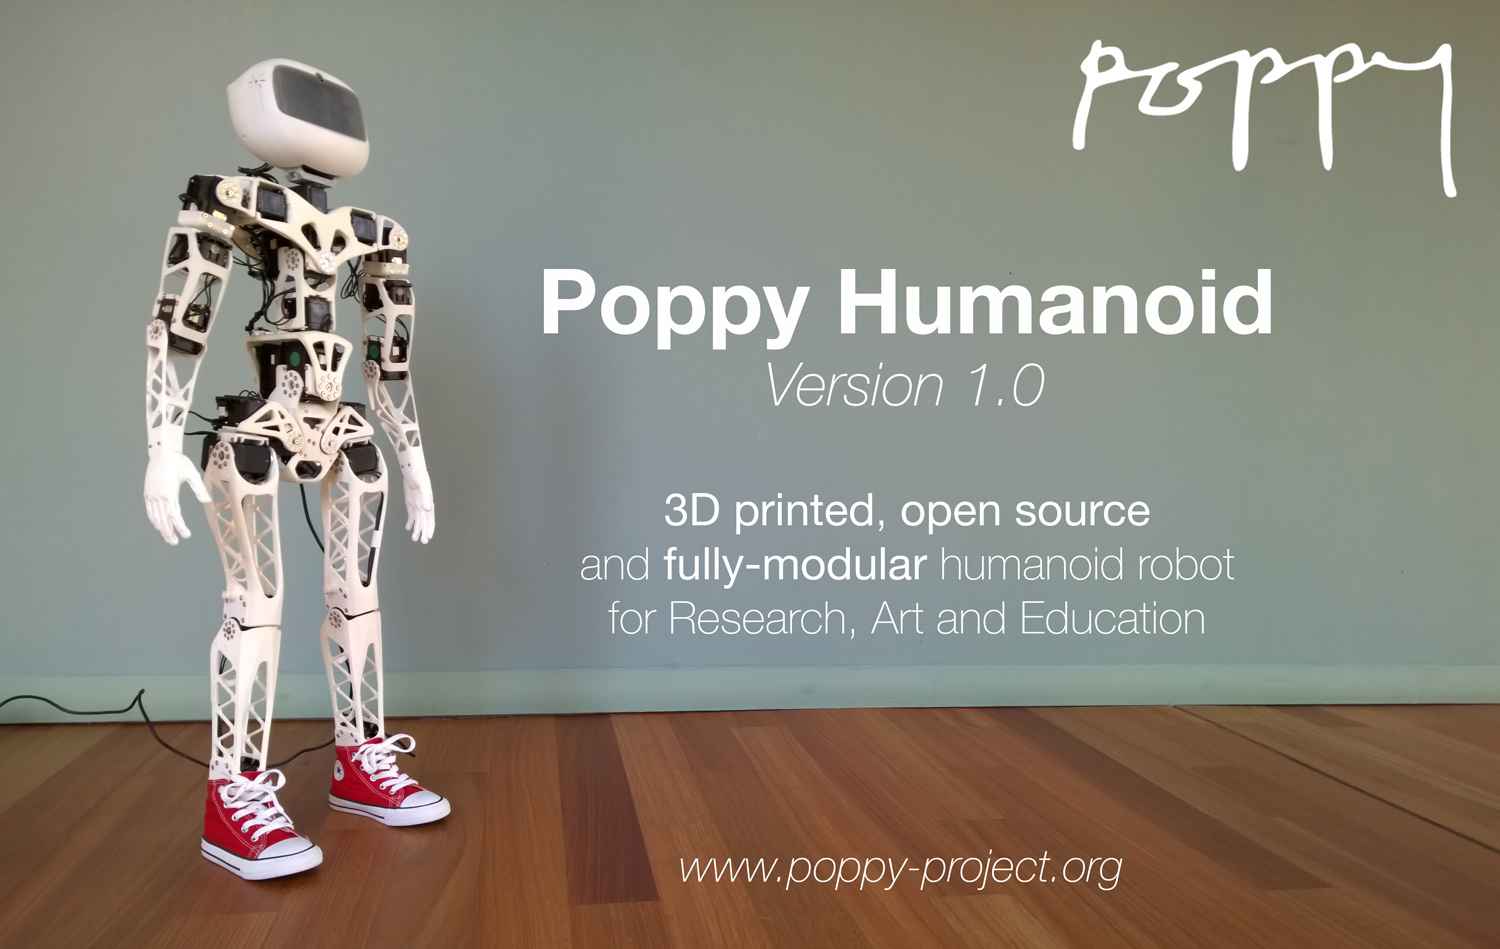
\includegraphics[width=0.9\linewidth]{poppy-humanoid-v1.jpg}
      \end{center}
      \caption{}
      \label{fig:poppy_humanoid_v1}
  \end{figure}

Le robot Poppy Humanoid v1.0 fait 85cm de haut et est particulièrement léger (3,5 kg). Ce robot dispose de 25 degrés de liberté avec un tronc multi-articulé (5 DoFs). Sa structure mécanique est entierement imprimée en 3D. Il est actuellement mis en mouvement par des servomoteurs Robotis, permettant d'avoir des réactions compliantes aux des forces extérieures, mais l'utilisation de servomoteurs alternatifs est actuellement explorée par la communauté\footnote{\url{https://forum.poppy-project.org/t/is-it-possible-to-replace-robotis-actuators-by-cheaper-ones/128}}.
Pour le contrôle embarqué il y a une ODROID U3 située dans la tête, permettant d'exectuer du code python et de gerer la communication (ethernet et Wifi).
Les capteurs comprennent une webcam grand angle située dans la tête qui peut être utilisée pour explorer la vision artificielle, ainsi que tous les capteurs embarqués sur les moteurs Robotis (capable de détecter la position, la vitesse, la charge ou encore monitorer la température).

Toute sa structure peut être reconfigurée pour modifier, remplacer ou supprimer des parties de son corps où l'une de ces caractéristiques. Sa morphologie de base est inspirée par la morphologie fonctionnelle humaine: un grand nombre d'articulations (25 moteurs), proportions, colonne vertebrale multi-articulé, femurs inclinés de manière similaire à ceux de l'homme...


La plate forme est totalement open source et ses fichiers sont distribués sur un dépot GitHub (voir \url{https://github.com/poppy-project/poppy-humanoid/} qui contient:

\begin{itemize}
  \item le package Python poppy\_humanoid,
  \item les fichiers CAO (Solidworks, STEP, Parasolid),
  \item le modèle URDF pour l'utilisation dans un simulateur (en particulier vrep) 
  \item et la documentation complète pour construire le robot (voir \url{https://github.com/poppy-project/poppy-humanoid/blob/master/hardware/doc/Poppy_Humanoid_assembly_instructions.md}).
\end{itemize}

La description plus complète et détaillée de la plate-forme est disponible en anglais chapitre~\ref{cha:poppy-dev}.



\section*{Applications} % (fold)


\subsection*{Exploration du rôle du corps} % (fold)
Poppy a été conçu pour être une nouvelle plate-forme expérimentale ouvrant la possibilité d'étudier de manière systemique le rôle de la morphologie sur le contrôle sensori-moteur, l'interaction homme-robot et le développement cognitif. En effet, comme nous en avons discuté, une conception appropriée de la morphologie d'un robot peut grandement simplifier les problèmes de contrôle, augmenter la robustesse, et ouvrir la voie à de nouveaux modes d'interaction avec le monde physique et social. Ainsi, être en mesure d'étudier le corps comme une variable expérimentale, quelque chose qui peut être facilement changée et expérimenté, est d'une importance primordiale. Pourtant, jusqu'à recemment, cela était compliqué car la construction d'un robot reposait sur des techniques de fabrication lourdes et coûteuses, mais l'impression 3D a changé le champ des possibles.

\begin{figure}[!t]
\centering
    \subfloat[][bended thighs]{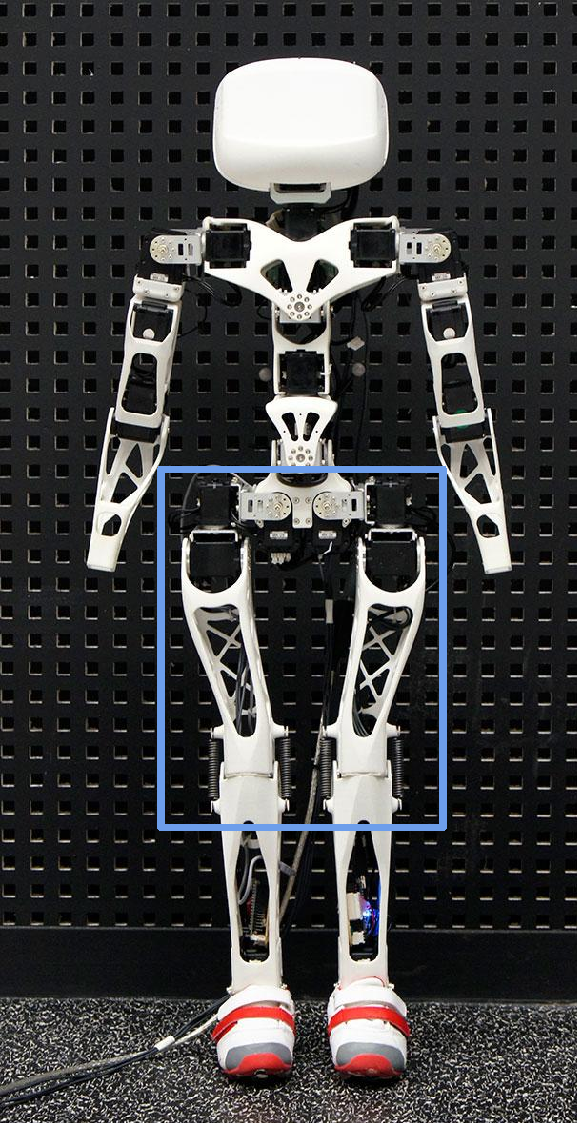
\includegraphics[width=0.35\linewidth]{poppy_bended_tigh_square.pdf}}
    \hfil
    \subfloat[][straight thighs]{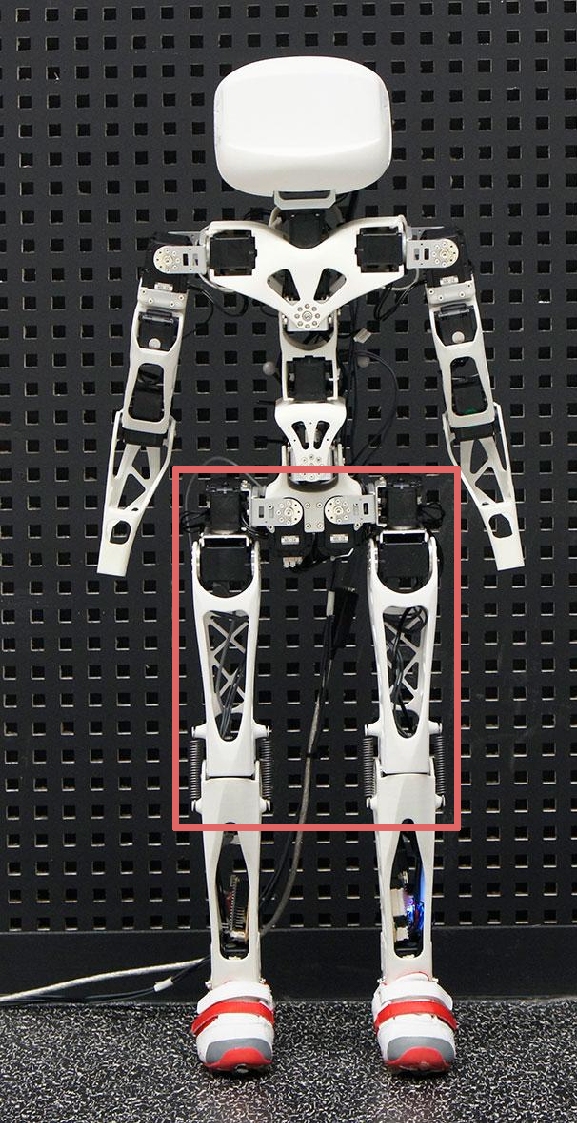
\includegraphics[width=0.35\linewidth]{poppy_straight_tigh_square.pdf}}
    \caption{Example de modification de la morphologie de Poppy. Ici l'architecture modulaire permet de remplacer les cuisses de Poppy et de comparer 2 configurations, une bio-inspirée (à gauche) et une plus traditionnelle (à droite)}
\end{figure}

Nous avons introduit une méthodologie de conception reposant sur l'utilisation de composants standards, d'une architecture électronique Arduino, combinés avec l'impression 3D qui joue un rôle central dans la production de pièces mécaniques de Poppy.

Il est maintenant possible d'explorer de nouvelles formes du corps en quelques jours. En plus de sa taille et de sa faible masse, la puissance des moteurs utilisés réduit fortement le risque de s'auto-dommager en cas d'erreur de programmation. Ce qui signifie que l'expérimentation peut être directement réalisée dans le monde réel, sans avoir à utiliser un simulateur ou construire un dispositif de sécurité.

Dans cette thèse nous présentons differentes experiences dont le but est de montrer à travers quelques examples qu'il est en effet possible de rapidement et facilement "hacker" la plate-forme Poppy pour explorer differentes variations morphologiques et les experimenter dans le monde réel. 
Les examples suivants sont présentés:
\begin{description}
    \item[Exploration du rôle de la morphologie]: Dans cet example, nous avons étudié l'impact de la forme de la cuisse bio-inspirée (inclinée de 6 degree) sur la stabilité durant la locomotion bipède. Nous comparons cette conception avec une cuisse droite plus traditionnelle. Nous décrivons à la fois le modèle théorique et des experiences réelles qui montrent que, durant la marche, la cuisse de bio-inspirée réduit la vitesse de chute laterale de près de 60\% (phase d'appui simple) et diminue le mouvement latéral nécessaire pour transferrer la  masse d'un pied sur l'autre de 30\% (phase d'appui double). Nous présentons également une expérience où le robot marche sur un tapis roulant aidé par un utilisateur expert et nous montrons que la cuisse bio-inspirée réduit les mouvements du haut du corps d'environ 45\% indiquant une démarche plus stable. Pour les details, voir section~\ref{sec:morphology-role}).

    \item[Fast exploration of morphological variants] Dans cette example, nous avons décidé de mener une expérience sur plusieurs variations de la morphologie du pied comme une illustration de la méthodologie que nous avons initié avec Poppy.
    Le but de cette expérience est d'explorer rapidement l'effet de la morphologie du pied sur sa stabilité. Ici, nous sommes particulièrement intéressés à la stabilité de la tête après un impact du pied. Ces impacts sont assez difficile à simuler de façon réaliste et la compliance naturel de la plate-forme Poppy rend d'autant plusimportant le fait d'experimenter sur le robot réel plutôt qu'avec un simulateur. Pour les details de l'experience, vous referer à la section~\ref{sec:morphology-variable}.
    \item[Adding new sensors to Poppy:]Lors de nos premiers essais pour concevoir une primitive de marche, nous nous sommes intéressés à la mesure de la pression sous les pieds. Cependant, la plate-forme de base de Poppy ne comporte pas de tels capteurs. Avec une plate-forme robotique traditionnelle, nous devrions soit utiliser les capteurs disponibles \emph{(dans ce cas la mesure très peu fiable de la charge du moteur Dynamixel de la cheville)}, ou ajouter un périphérique externe avec son propre système d'alimentation électrique et de communication.

    Grace à la modularité électronique et logicielle de Poppy, nous pouvons "hacker" le robot et intégrer de nouveaux capteurs. Ensuite, ils peuvent être branchés sur la carte electronique embarquée.

    Pour donner un exemple de la façon dont nous pouvons réellement "hacker" le robot Poppy, nous expliquons dans cette example comment nous avons fait pour intégrer des capteurs de force sous les pieds de Poppy et enregistré les données avec la bibliothèque de pypot, voir section~\ref{sec:morphology-adding-sensors}.
\end{description}

\subsection*{Artistique} % (fold)

Le travail des artistes est complémentaire de celle des scientifiques. En effet, la communauté artistique est une riche source d'inspiration et peut offrir de nouvelles perspectives sur des questions scientifiques et technologiques. 
Poppy étant totalement "hackable", nous pensons que les artistes peuvent se l'approprier et le modifier selon leur besoins. De plus, il est conçu pour être resister aux expérimentations, sa robustesse et sa facilité de reparation font en sorte qu'il peut être utilisé dans des conditions assez difficiles.

Dans la communauté robotique open source que nous essayons de mettre en place, cette complémentarité est une grande opportunité que nous voulons encourager en faisant de Poppy, un robot accessible pour les utilisateurs non-experts en robotique.

Bien qu'il soit un vrai désir de faire Poppy accessible et utile pour la communauté artistique, nous avions besoin d'acquérir de l'expérience de ces utilisations dans un projet artistique réelle afin d'évaluer si l'utilisation de Poppy est pertinente pour des artistes et explorer ce que les artistes peuvent apporter à son développement.


Le premier projet artistique dans lequel est impliqué Poppy est intitulé "Êtres et Numérique". Ce projet d'art contemporain se concentre sur les façons de représenter et d'interagir avec le mouvement numérique. Il est dirigé par les artistes\footnote{Comacina Capsule Creative,\url{http://www.comacina.org/}} Amandine Braconnier (artiste plasticienne) et Marie-Aline Villard (danseuse-chercheuse), et supervisé par Thomas Desmaison (point barre\footnote{\url{http://www.pointbarre.biz/}}) de la Fabrik Pola \footnote{\url{http://www.pola.fr/}}.


Pour ces artistes, l'utilisation d'un robot humanoïde hackable est un outil d'expression qui ouvre de nouveaux horizons. En effet, un robot permet de disséquer et analyser les mouvements. Il leur permet de jouer avec son corps et de modeler ses gestes comme sculpter des formes en argile. En outre, l'utilisation d'un actuation compliante permet l'émergence de mouvements imprévisibles et inattendus, tout en assurant une intéraction physique directe sûre.

Le premier projet d'"Êtres et Numérique" a pris la forme d'une résidence art-science-médiation de dix jours impliquant des membres du projet Poppy, les artistes avec la participation de Jean Marc Weber (compositeur de la musique) et a été soutenu par la Région Aquitaine. Elle a eu lieu à Bordeaux(Fr) dans le Lycée Sainte-Famille Saintonge\footnote{\url{http://www.lyceesaintefamille.com/}}), qui a fait de sa magnifique chapelle un salle pour les spectacles artistiques. \textbf{Un trailer vidéo de cette résidence est disponible ici: \url{https://vimeo.com/92281019}.}


Le travail que les artistes ont fait a été vraiment incroyable et elles ont trouvé un potentiel inattendu dans Poppy. En particulier, la chorégraphie que Marie Aline Villard a fait est très élégante et sensible. Ces mouvements mettent Poppy dans une domaine de sensibilité rarement vu en robotique humanoïde. Cette chorégraphie est maintenant souvent utilisée pour la démonstration de la plate-forme Poppy et cloture la video de montage en time-lapse \url{https://vimeo.com/96262428}.

Pour une description et un retour detaillés des experiences artistiques qui ont eu lieu durant cette thèse, vous reporter au chapitre~\ref{cha:art}.

\subsection*{Education} % (fold)
Les technologies liée au prototypage rapide, à l’impression 3D et au DIY (Do it Yourself) n’ont pas simplement aujourd’hui un impact dans les laboratoires, mais sont au coeur d’une révolution sociétale en marche, que d’aucuns nomment la révolution des « makers », et qui bouleverse les modes de design et de fabrication dans l’industrie. Aujourd’hui les plus grands groupes commencent à concevoir et à construire des voitures, des avions, des bâtiments imprimés en 3D. Des start-ups nombreuses se développent grâce à des technologies rendues possibles avec l’impression 3D, et souvent créées par une population de « jeunes geeks », qui se sont formés dans des FabLabs, ces nouveaux « garages » dans lesquels les passionnés apprennent et créent avec ces technologies. Outre l’impression 3D, l’intégration de composants hétérogènes et hackable, informatiques, électroniques et mécaniques, constitue une caractérisque essentielle de ce mouvement.

Hors cela pose un défi aux systèmes éducatifs, aux écoles d’ingénieurs en particulier, mais aussi aux structures de formation à l’intérieur des entreprises industrielles, que de transmettre ces nouveaux modes de conception, de la pensée à la fabrication. Avec cet objectif en tête, de nombreuses écoles, et les Fablabs eux-mêmes, lancent aujourd’hui des projets éducatifs dans lesquels les apprenants sont amenés à concevoir, modifier, expérimenter eux mêmes selon cette approche.

Par ses propriétés, la plateforme Poppy répond aussi a un besoin sociétal grandissant : l’éducation et la formation aux technologies mêlant informatique, électronique et mécanique, ainsi que la formation à l’outil de prototypage révolutionnaire qu’est l’impression 3D. Par son ouverture, son coût modeste et son design, Poppy fournit un objet et un contexte unique pour permettre l’expérimentation et l’apprentissage de ces technologies selon une approche « Do It Yourself ».

Plusieurs expériences avec Poppy dans des collèges, des lycées, des Fablabs et des musées de Sciences en France et à l’étranger ont eu lieu durant cette thèse ou vont avoir lieu.

En particulier, cette thèse presente 2 experiences qui ont été une chance pour faire un veritable crash-test de la plate-forme dans des conditions écologiques (en milieu réel et utilisateurs non-experts)):
\begin{enumerate}
    \item La première s'est déroulée lors d'un "hackathon" organisé par la Cité des Sciences dont le but était de faire construire le Poppy du Fablab par le grand public. Sans personne de notre équipe présente, le d'une dizaine de personnes de tout ages a réussi à monter et rendre fonctionnel une version beta de Poppy dans le temps du WE. Le support live étant assuré via la plate-forme d'échange (forum) Poppy.
    \item La seconde a été une exploration pédagogique avec des élèves de seconde STI-2D du Lycée Saintonge Sainte Famille à Bordeaux. Cette fois ci organisé sur 3 demi journées et differents ateliers, les étudiants ont assemblé un buste de Poppy (moins cher qu'un humanoide complet) et appris à le programmer en python avec pypot.
\end{enumerate}


Ces 2 experiences ont été très instructives et ont posé les bases d'une proposition de projet FEDER "Poppy Education" qui nous avons formulé et qui a été accepté par la région Aquitaine pour financer le developpement d'outils dédiés à l'utilisation de Poppy dans le milieu éducatif (lycée et post-bac).

Les détails de ces experiences et les retours que nous en avons tirés sont décris dans le chapitre~\ref{cha:education}.


\section*{Conclusion: contributions de cette thèse} % (fold)

Tous les aspects de la plate-forme Poppy ont été conçus pour être très modulaire, hackable, robuste et facile à reproduire dans le milieu académique afin de faciliter le developpement cumulatif et la reproductibilité scientifique. En quelques jours, nous pouvons maintenant étudier de manière systemique la façon dont différentes formes des jambes ou des pieds peuvent influencer l'équilibrage ou la locomotion bipède, ou étudier les réactions que peuvent provoquer différentes morphologies de la tête lors d'interactions social avec l'homme.

Poppy a d'abord été présentée comme une de plate-forme facilement modifiable à la conférence AMAM2013~\parencite{lapeyre:hal-00788433}, sa conception a été expliqué plus en détail pour IROS 2013~\parencite{lapeyre:hal-00852858} ainsi que sa pertinence potentielle pour explorer l'interaction sociale~\parencite{lapeyre:hal-00984312}. Ensuite, nous avons mené plusieurs expériences pour démontrer ses propriétés uniques. D'une part, en explorant le rôle de la morphologie de la cuisse sur la dynamique de la marche bipède, présenté à Humanoids2013~\parencite{lapeyre:hal-00861110}. D'autre part, en démontrant qu'il est possible de faire de la morphologie une variable expérimentale. Des expériences ont été menées pour tester différents modèles de pieds et ont été présenté à Humanoids2014~\parencite{lapeyre2014humanoids}.

Deuxièmement, la distribution open source a attiré une attention particulière, qui nous a permis de commencer la création d'une communauté multidisciplinaire. Grâce à l'interet que nous avons réçu, nous avons trouvé des acteurs éducatifs et des artistes désireux d'explorer de nouvelles applications avec des robots. Ce travail nous a conduit à mener plusieurs expériences très instructives et a ouvert de nouvelles perspectives pour l'utilisation de Poppy dans l'Art et l'éducation; un papier associé a été publié pour DI2014~\parencite{lapeyreDI}.

Cependant, une des contributions principales a certainement été la distribution open source du premier robot humanoide complet à être à la fois imprimé en 3D et open source, qui peut être utilisé librement par quiconque comme une plate-forme expérimentale. 
Ce robot participe au mouvement d'open science qui manque d'outils disponibles et accessibles pour les chercheurs en robotique.  Maintenant même ceux travaillant sur les problématiques hardware peuvent partager leur travail avec la communauté scientifique. En outre, Poppy offre une alternative aux laboratoires désireux d'expérimenter dans le monde réel. Ils ne sont plus contraints d'acheter un robot soit fermée et limitée, ou d'investir des ressources dans le développement d'une nouvelle plate-forme expérimentale, ils peuvent choisir d'utiliser le travail déjà fait avec Poppy et l'adapter selon leurs besoins.
Plusieurs laboratoires de recherche en Europe ont déjà commencé à utiliser la plate-forme de pavot pour leurs propres projets (par exemple, Collège de France, Bristol Robotics Lab., Inria Nancy ...) ainsi que plusieurs écoles d'ingénieurs qui l'ont inclu dans leurs formations.

Enfin, concernant l'impact societal de cette thèse, les possibilités nouvelles ouvertes par le projet Poppy ont entrainé la création directe de 6 emplois qualifiés (sur le centre Inria Bordeaux) et de manière indirect genère de nouvelles activités dans plusieurs laboratoires, écoles (projets étudiants) et lieux publiques de création et diffusion scientifique (musée, fablabs,...).

Nous travaillons maintenant à faire émerger un éco-système ouvert autour des technologies open source Poppy et d'une communauté multi-disciplinaire actives avec comme objectifs le developpement des pratiques open science dans la communauté robotique et la mise en place d'outils pédagogiques pertinent pour l'apprentissage des sciences et de la programmation à l'école.





